\documentclass[a4paper,12pt]{article}
\usepackage[T1]{fontenc}
\usepackage[utf8]{inputenc}
%\usepackage[ngerman]{babel}
\usepackage{marvosym}
\DeclareUnicodeCharacter{20AC}{\EUR}
\usepackage{lmodern}

\usepackage{amsmath}
\usepackage[pdftex]{graphicx}
\usepackage{float}
\usepackage[format=hang, font={footnotesize,sf},labelfont={bf},margin=1cm, aboveskip=5pt, position=bottom]{caption}
\usepackage{multirow}
\usepackage{array}
\usepackage{makecell}
\usepackage{setspace}
\usepackage{xpatch}
\xpatchcmd{\thebibliography}{\section*}{\section}{}{}
\usepackage{cancel}
\usepackage{caption}
\usepackage{subfigure} %用于并排图片


\begin{document}

\section{Euler algorithm}

In this 1D harmonic oscillator simulation the mass $m = 1$ and the Hooke's constant $k = 1$. Therefor the acceleration $a$ can be expressed as 

\begin{equation}
    a =\frac{d^2x}{dt^2} = - \frac{k}{m} x(t) = -x(t)
\end{equation}

And Euler algorithm can be implemented as the following two equations 

\begin{equation}
    \begin{aligned}
    x(t+\Delta t) &= x(t)+v(t)\Delta t \\
    v(t+\Delta t) &= v(t)-x(t)\Delta t        
    \end{aligned}
\end{equation}

The initial values are position $x(0) = 0$ and velocity $v(0) = 0$. After the implementation of Euler algorithm with step length $\Delta t = 0.1$ (a) and $\Delta t = 0.1$ (b) in figure\ref{x_v_Euler}.

\begin{figure}[!htbp]
    \centering
    \subfigure[$\Delta t = 0.1 $]{
        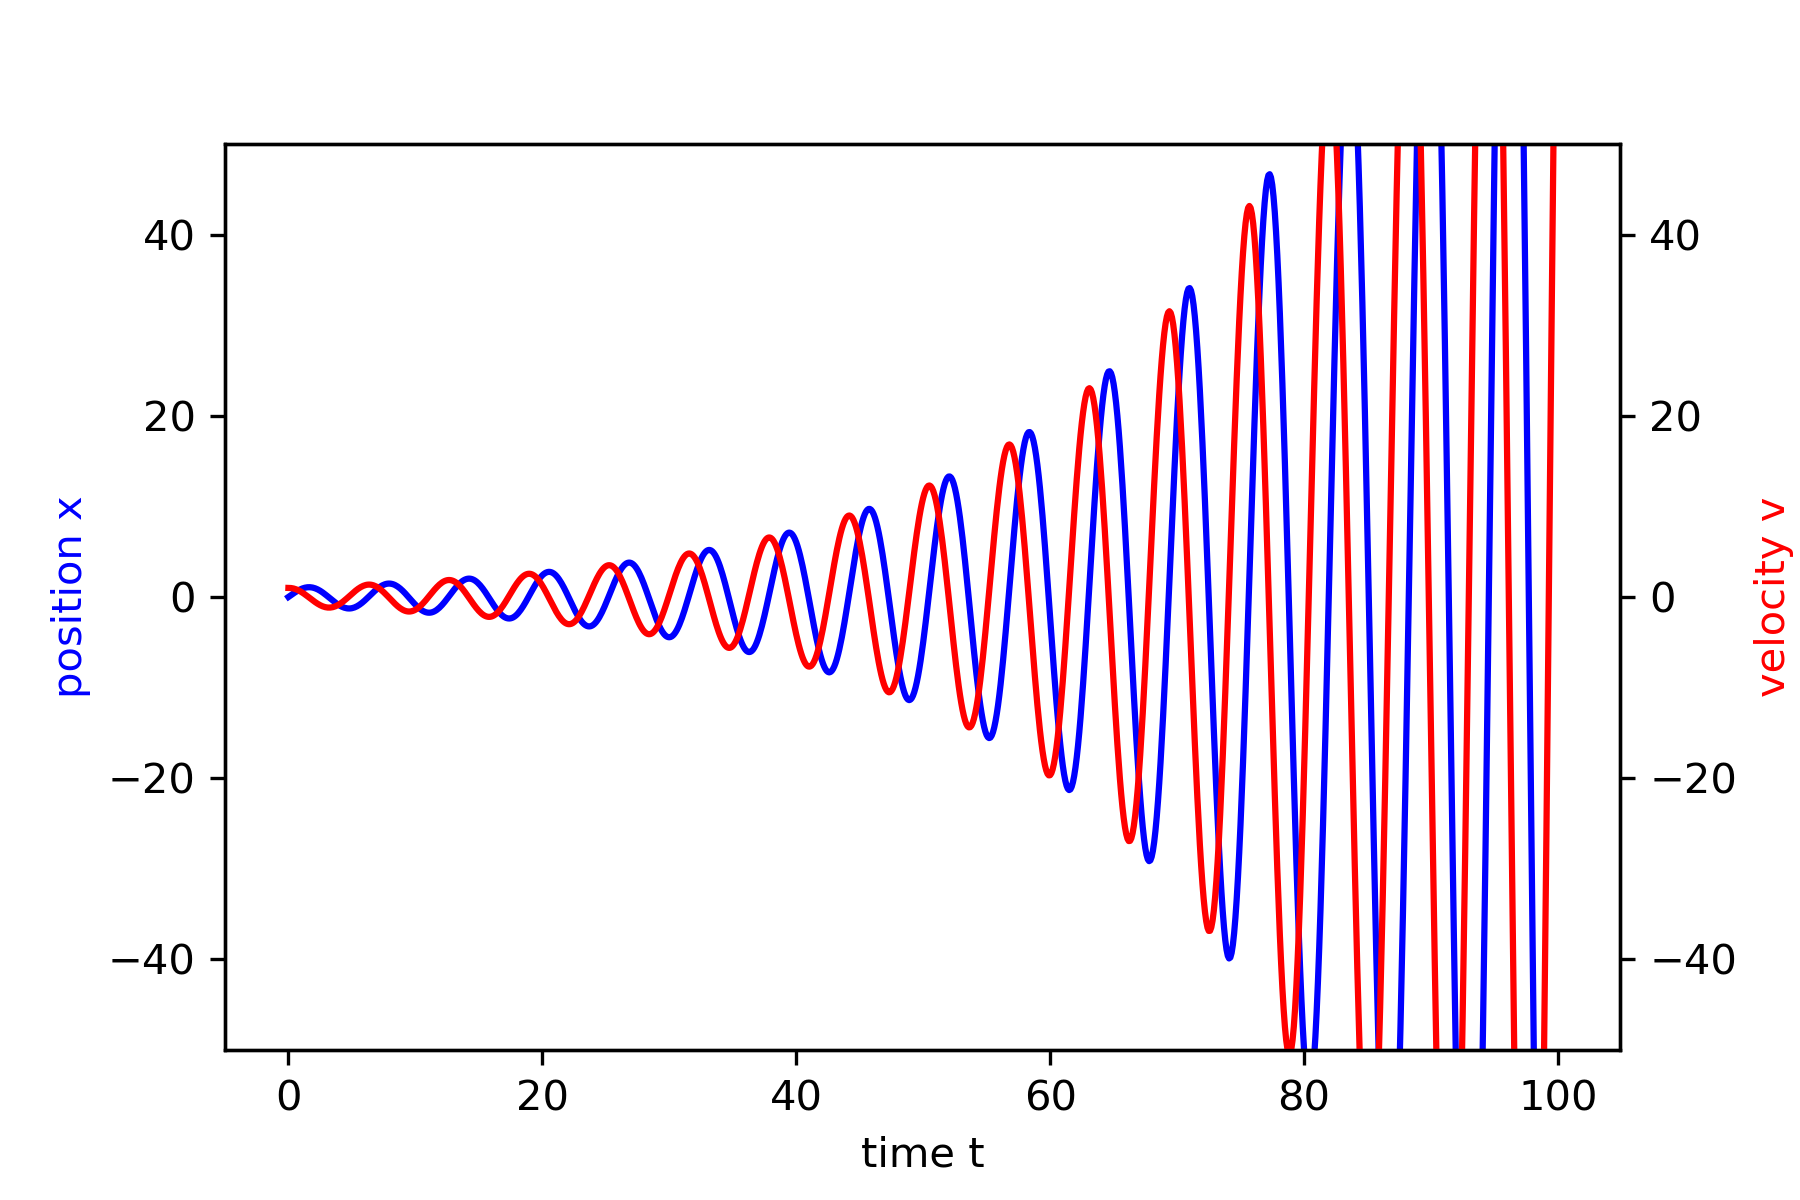
\includegraphics[width=6.5cm]{x_v_Euler01.png}
    }
    \subfigure[$\Delta t = 0.01 $]{
        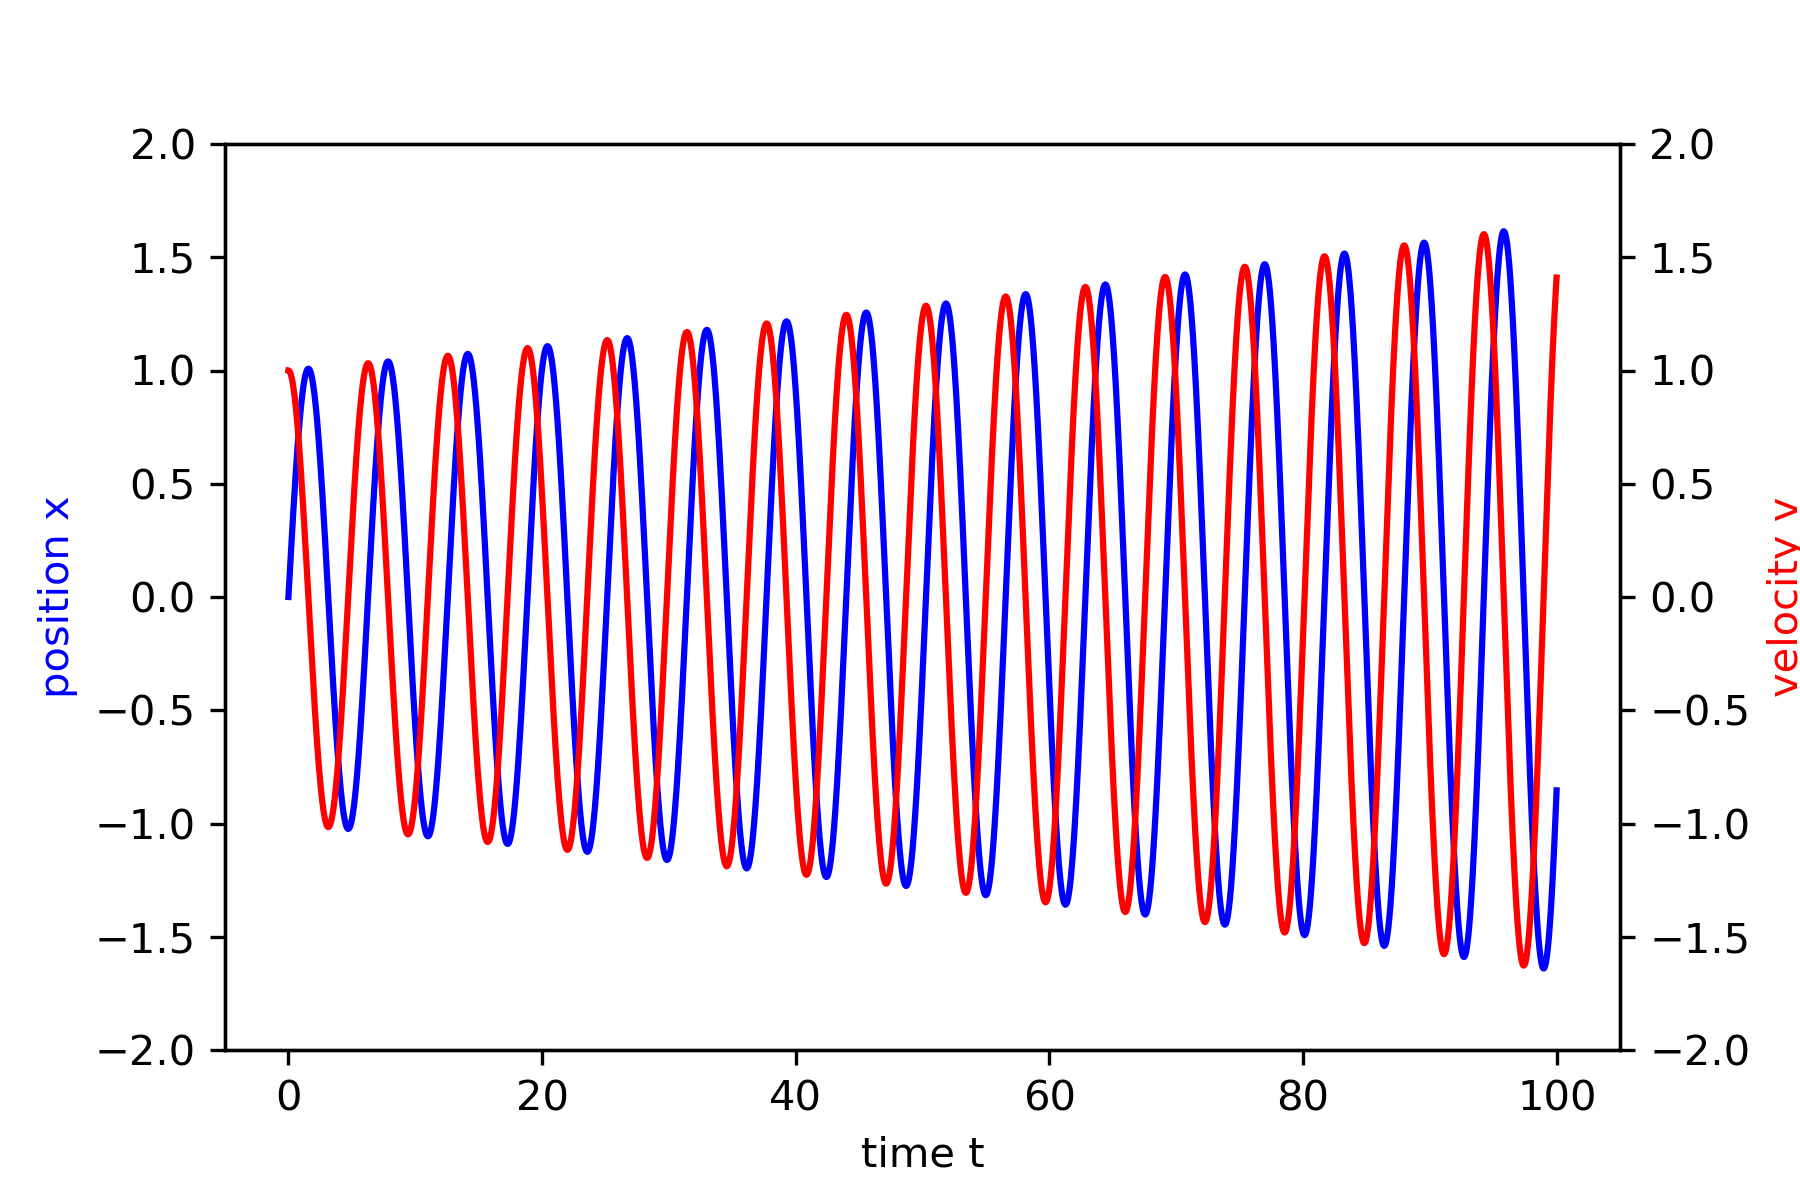
\includegraphics[width=6.5cm]{x_v_Euler001.png}
    }

    \caption{X-V-t diagram of Euler algorithm}
    \label{x_v_Euler}
\end{figure}

The energy can be calculated by 

\begin{equation}
    \begin{aligned}
        E &= \frac{1}{2} mv^2(t) + \frac{1}{2} k x^2(t)\\
        &= \frac{1}{2} (v^2(t)+x^2(t))
    \end{aligned}
\end{equation}

and the $Log(E) - t$ diagram is showed in Figure \ref{E_Euler}.

\begin{figure}[!htbp]
    \centering
    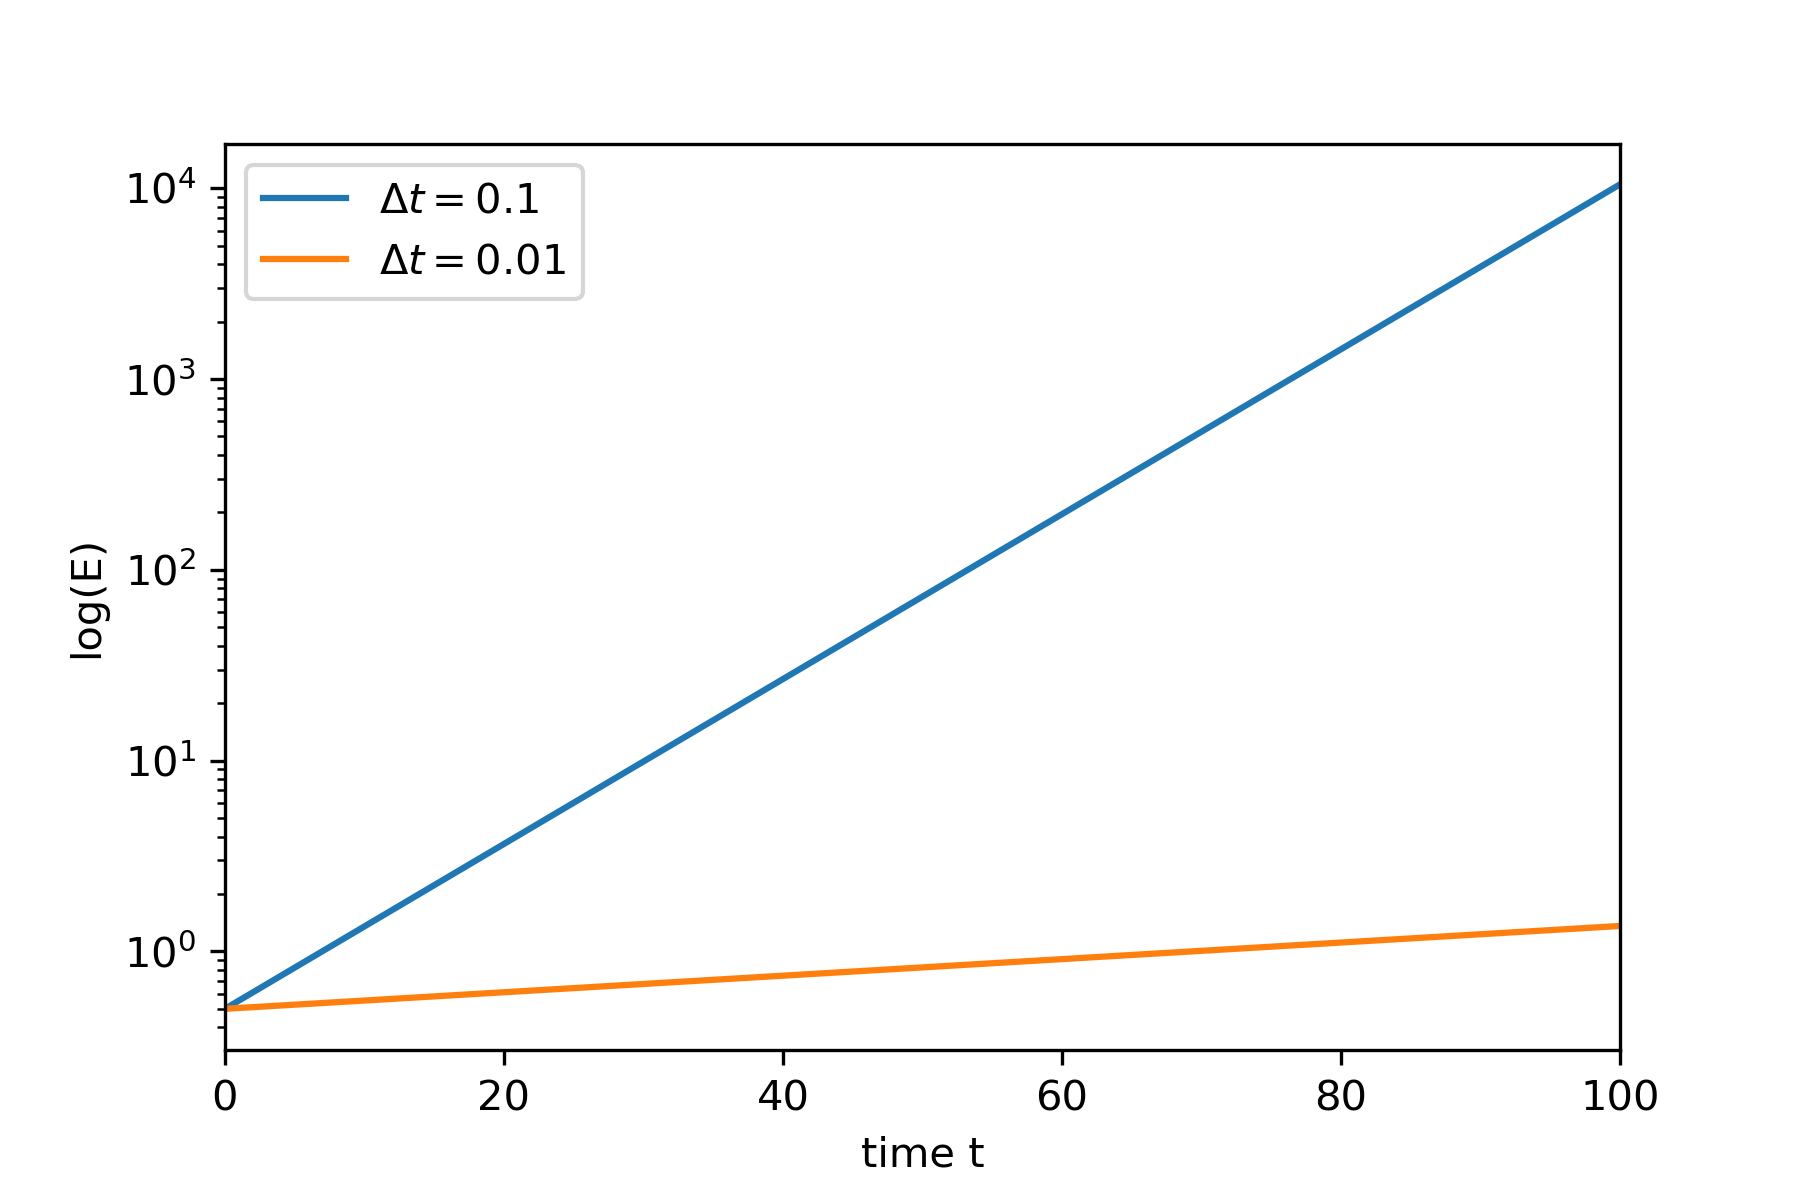
\includegraphics[width=10cm]{Euler_E.png}

    \caption{log(E)-t diagram of Euler algorithm}
    \label{E_Euler}
\end{figure}

the energy of the oscillator system is divergent with increasing steps of the calculation. When decrease the steps from 0.1 to 0.01, the divergence can be suppressed but not eliminated.

\section{Velocity-Verlet algorithm}

the Velocity-Verlet algorithm is implemented as

\begin{equation}
    \begin{aligned}
    x(t+\Delta t) &= x(t)+v(t)\Delta t - \frac{1}{2} x(t) \Delta t^2  \\
    v(t+\Delta t) &= v(t)-\frac{1}{2}(x(t+\Delta t)+x(t))\Delta t        
    \end{aligned}
\end{equation}

The initial values are still keep the position $x(0) = 0$ and velocity $v(0) = 0$. the result of x-t, v-t are showed in Figure \ref{x_v_VV} and energy E-t diagram in Figure \ref{E_VV}.

\begin{figure}[!htbp]
    \centering
    \subfigure[$\Delta t = 0.1 $]{
        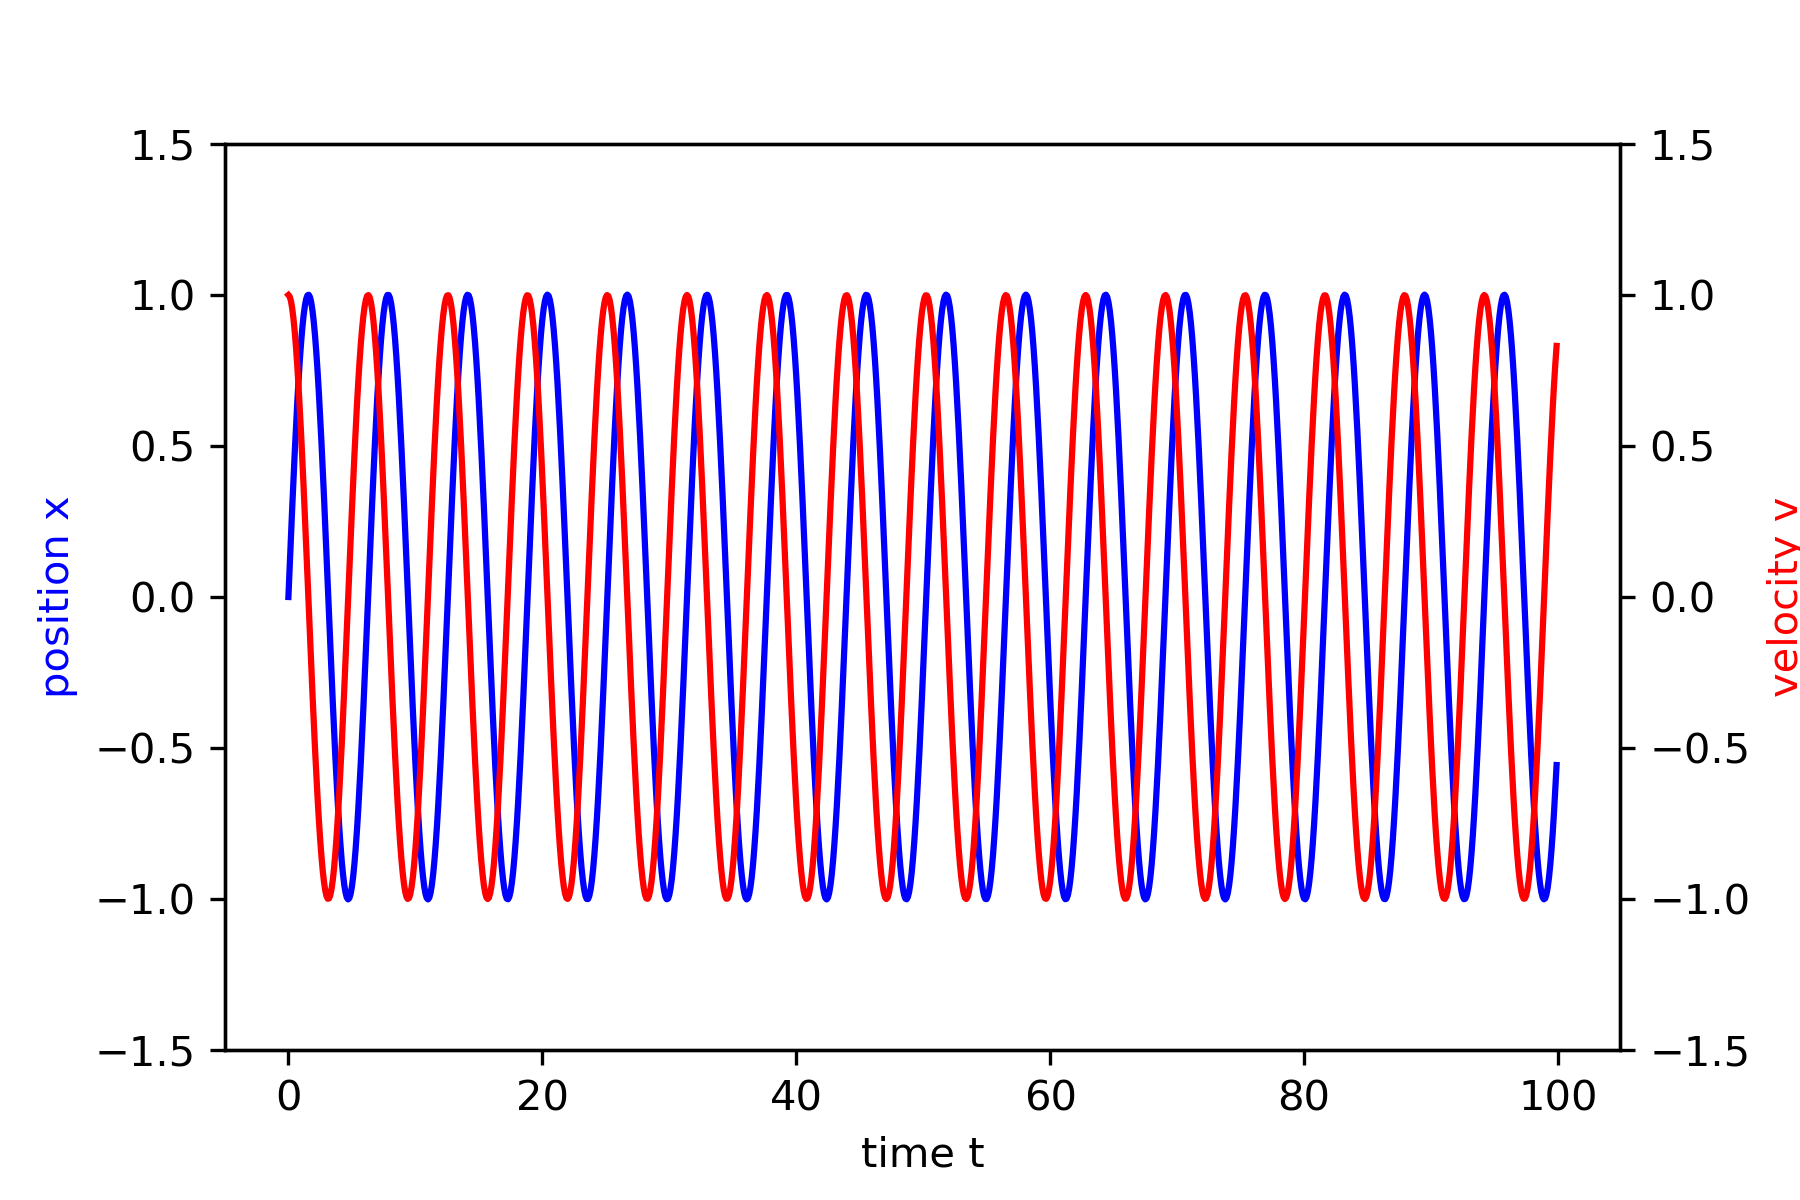
\includegraphics[width=6.5cm]{x_v_VV01.png}
    }
    \subfigure[$\Delta t = 0.01 $]{
        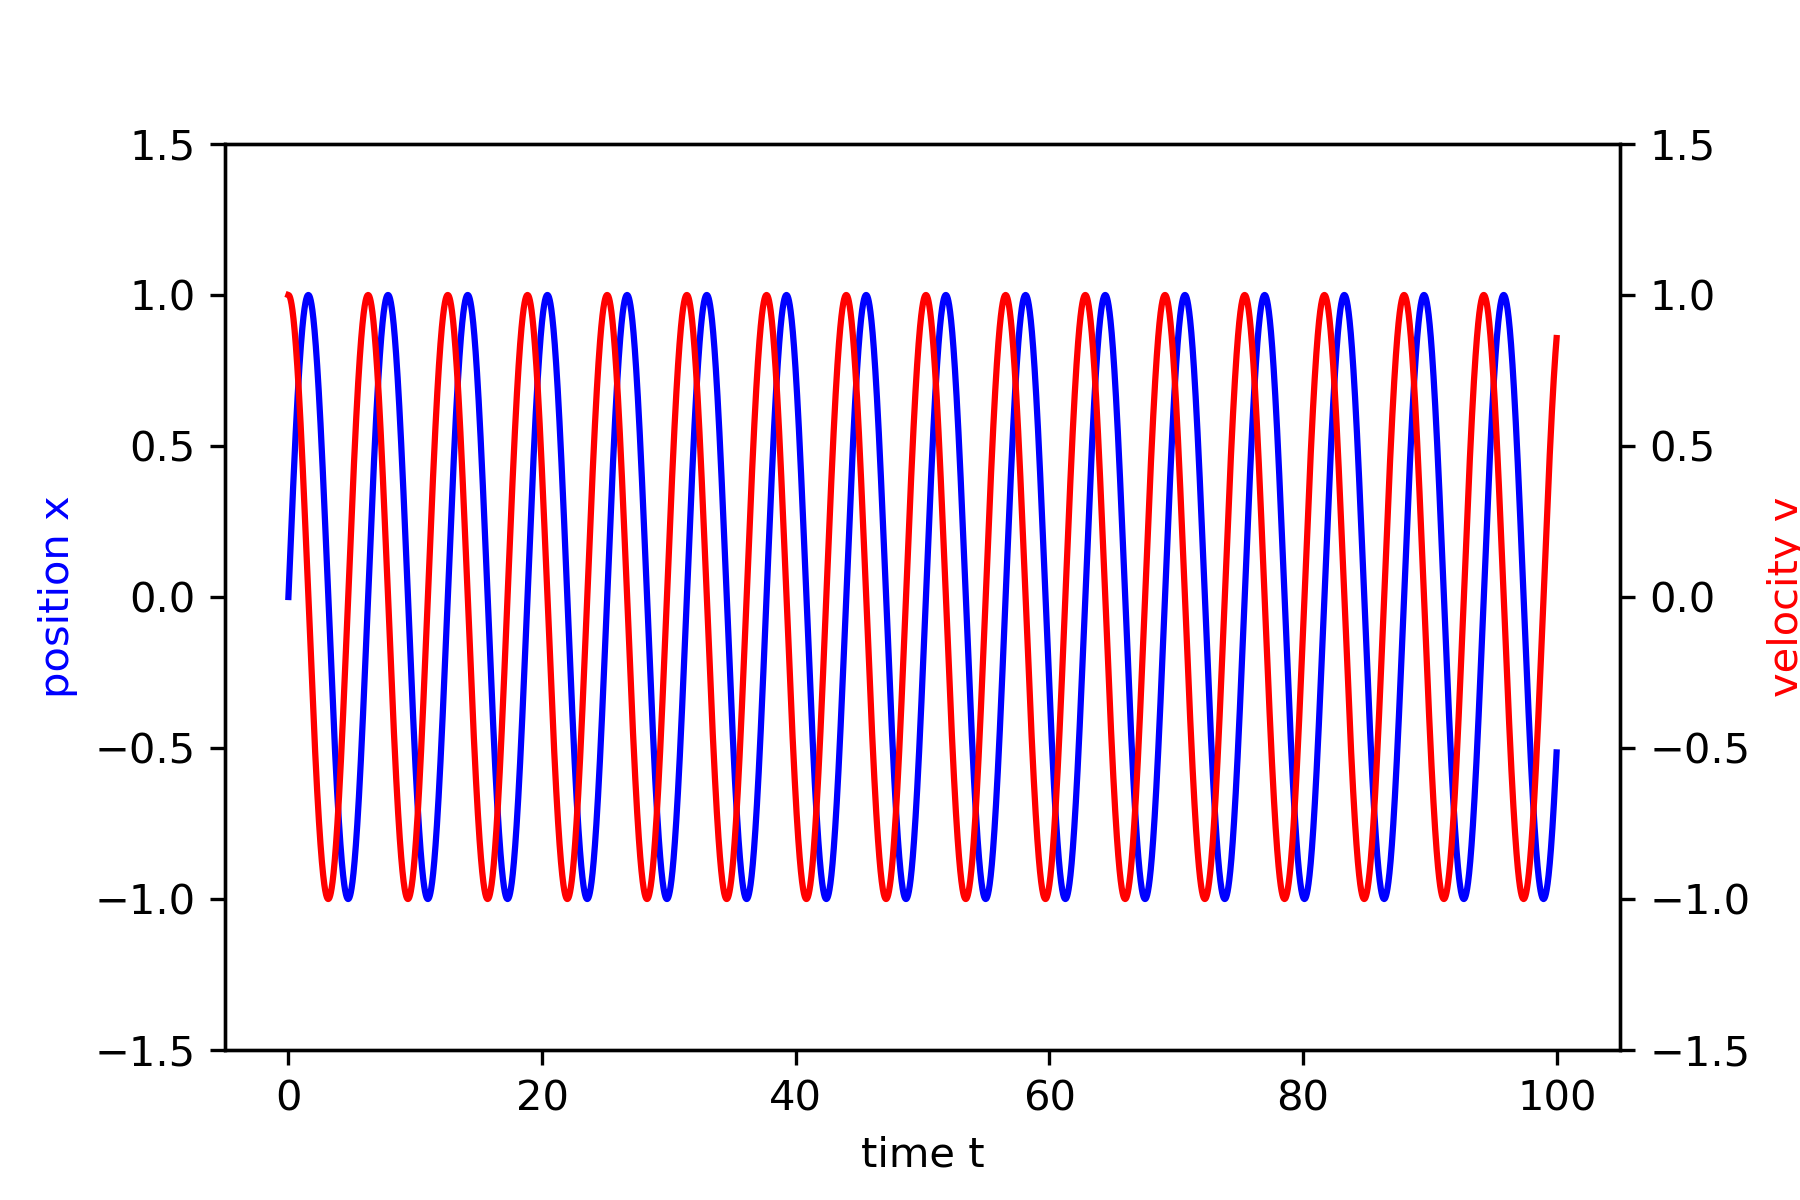
\includegraphics[width=6.5cm]{x_v_VV001.png}
    }

    \caption{X-V-t diagram of Velocity-Verlet algorithm}
    \label{x_v_VV}
\end{figure}

\begin{figure}[!htbp]
    \centering
    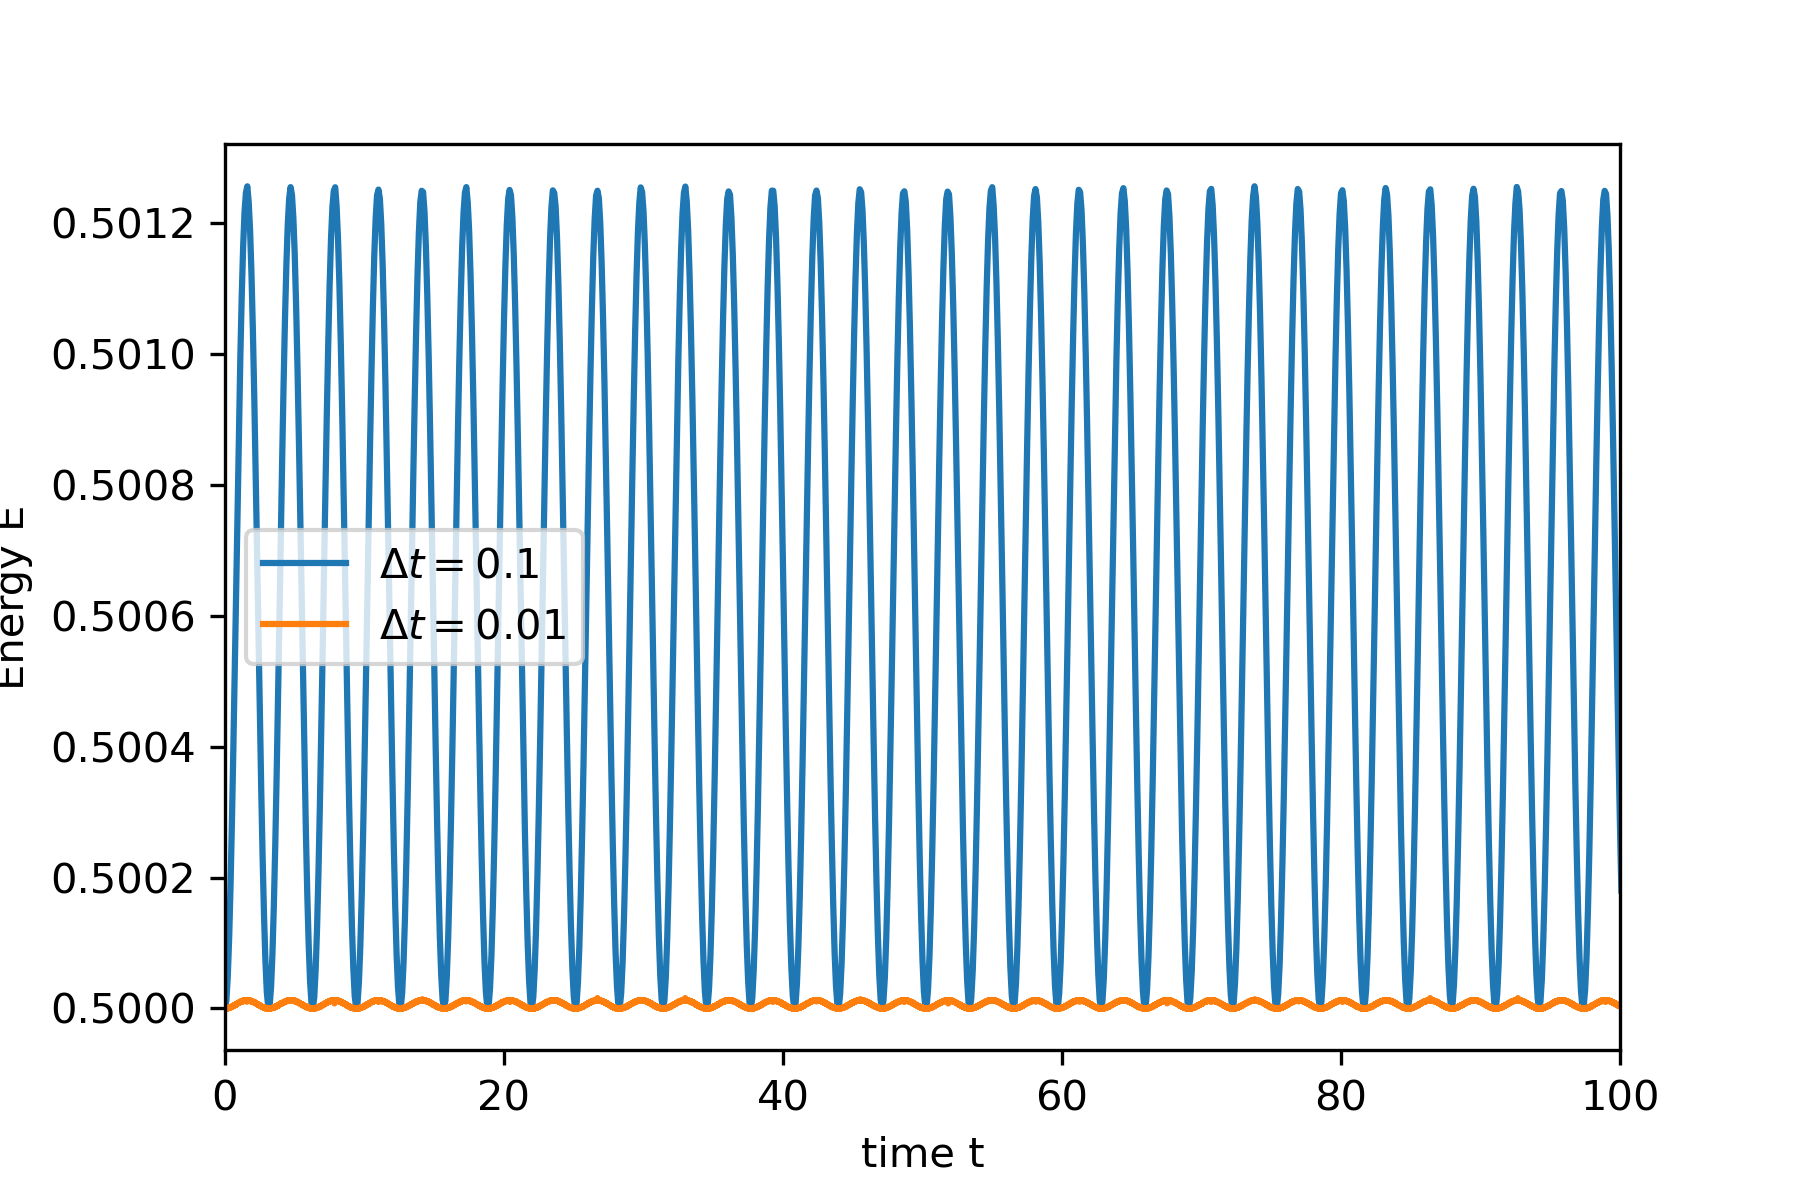
\includegraphics[width=10cm]{VV_E.png}

    \caption{E-t diagram of Velocity-Verlet algorithm}
    \label{E_VV}
\end{figure}

With the Velocity-Verlet algorithm the energy results are convergent. And shorter steps length is more stable.

\section{Differences between the Euler and the velocity-Verlet algorithm}

when the Euler and the velocity-Verlet algorithm compared with the analytic solution $x(t) = sin(t)$ (Figure \ref{x_t}), the results of velocity-Verlet algorithm is mach more better.

\begin{figure}[!htbp]
    \centering
    \subfigure[Euler algorithm]{
    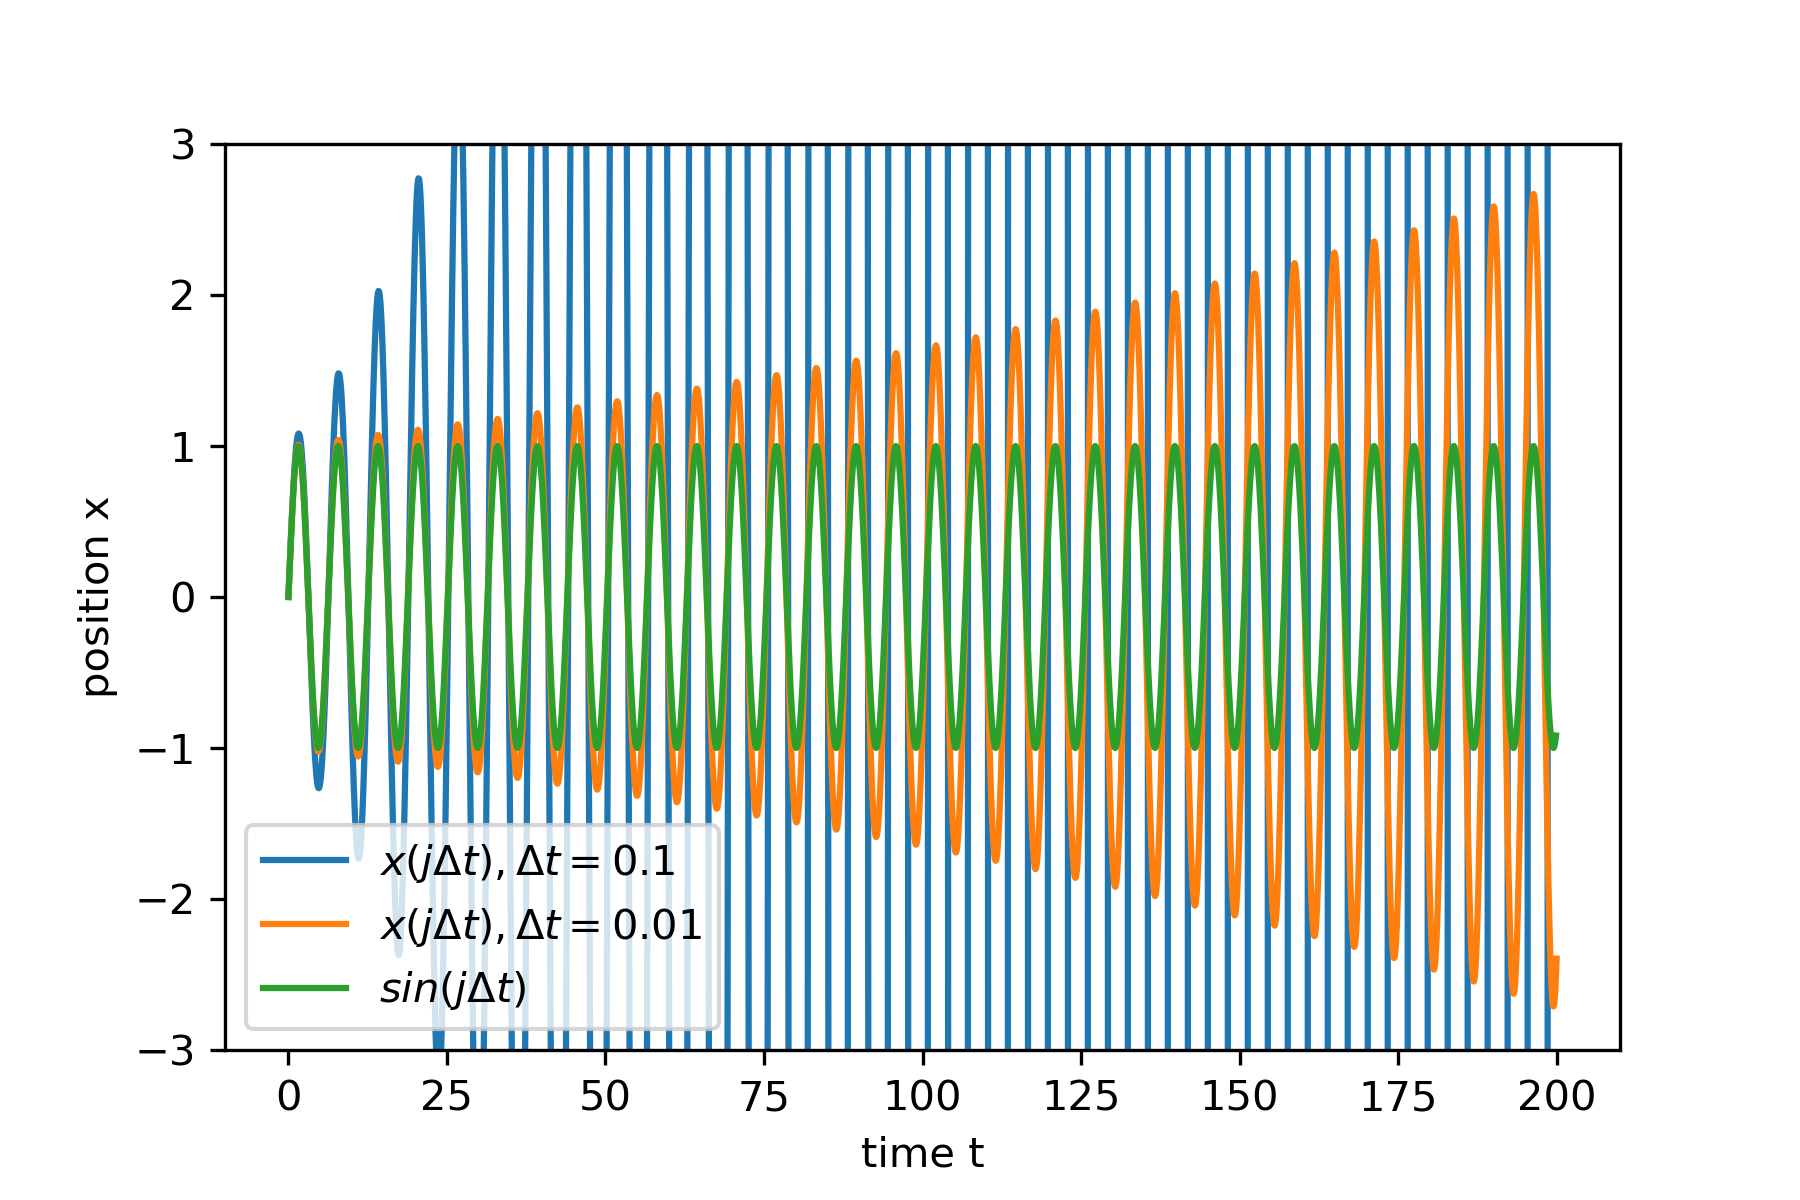
\includegraphics[width=6cm]{x_t_Euler.png}
    }
    \subfigure[Velocity-Verlet algorithm]{
    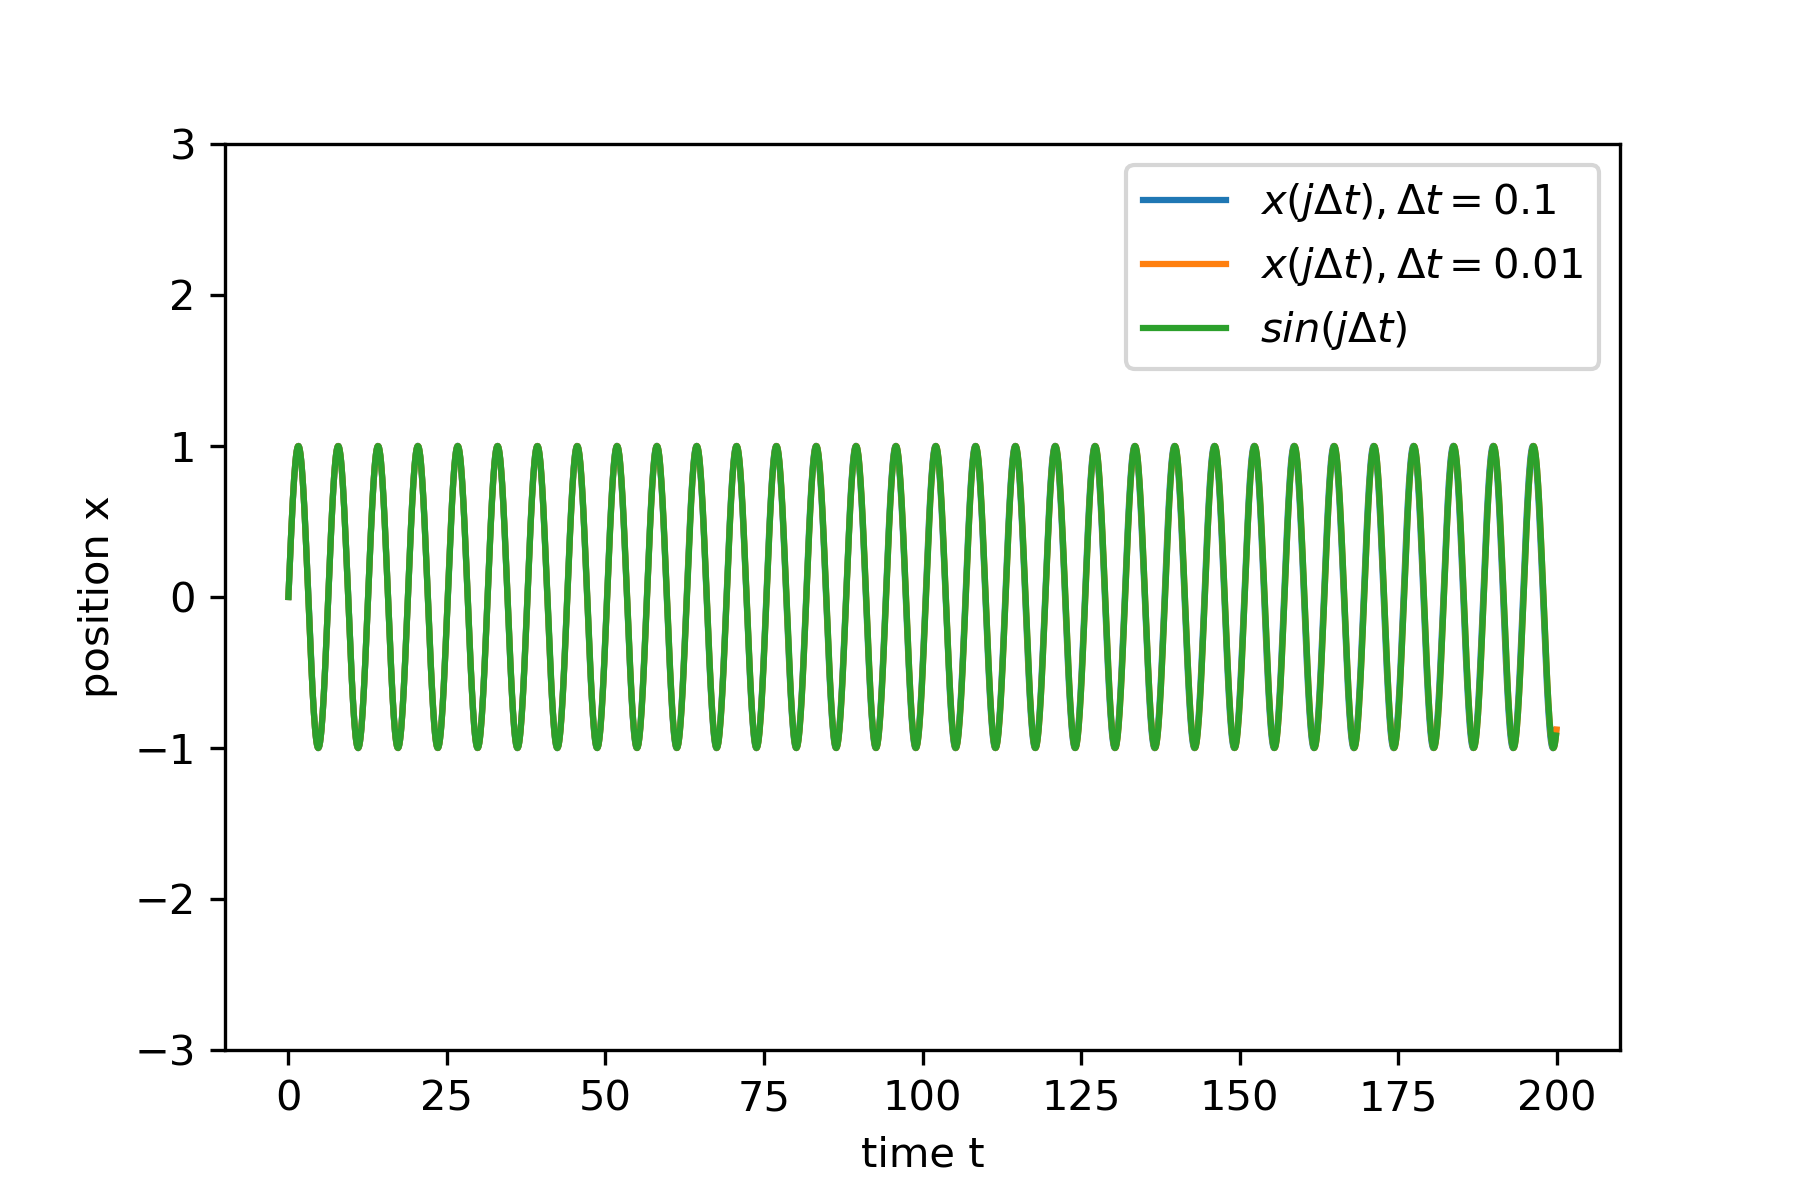
\includegraphics[width=6cm]{x_t_VV.png}
    }

    \caption{x-t diagram of Euler and Velocity-Verlet algorithm}
    \label{x_t}
\end{figure}

The Taylor expansion of position $x(t)$ is

\begin{equation}
    x(t+\Delta t) = x(t) + v(t)\Delta t + a(t)\Delta t^2 + O(\Delta t^3)
\end{equation}

Therefor the position $x(t)$ error of the Euler algorithm is second order $O(\Delta t^2)$. But for Velocity-Verlet algorithm the second order term is kept, the error is form $O(\Delta t^2)$.

When we focus on velocity equations of both algorithm, the Velocity-Verlet algorithm have the therm $x(t+\Delta t)$, which combined the latest step. It also help to get result, which closer to the facts.

\section{Summary}

Through implementation of Euler und Velocity-Verlet algorithm the sources of error are discussed. The step length, numerical carry and the simplify of equation will cause the error. Among them the simplify of equation of higher order tern play the most important row.

\end{document}